\subsubsection{UC7 - Acquisto beni}
\begin{figure}[h]
	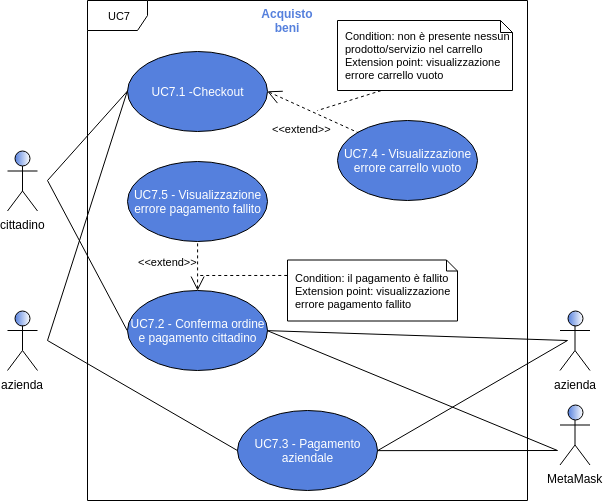
\includegraphics[width=10cm]{res/images/UC7-Generale.png}
	\centering
	\caption{UC7 - Acquisto beni}
\end{figure}
\begin{itemize}
	\item \textbf{Attori Primari}: cittadino e azienda-cliente;
	\item \textbf{Attori Secondari}: azienda-venditrice, MetaMask\glo;
	\item \textbf{Descrizione}: i cittadini e le aziende possono acquistare i beni/servizi che avevano precedentemente aggiunto nel carrello;
	\item \textbf{Scenario principale}: 
	\begin{enumerate}[label=\alph*.]
		\item l'utente procede con il checkout dei prodotti precedentemente inseriti [UC7.1];
		\item l'utente sceglie l'indirizzo di spedizione [UC7.3];
		\item l'utente effettua la conferma ed il pagamento dell'ordine [UC7.4].
	\end{enumerate}
	
	\item \textbf{Precondizione}: il sistema ha reso disponibile all'utente l'utilizzo del carrello per poter effettuare degli acquisti. L'utente ha inserito degli oggetti nel carrello ed effettua il procedimento di acquisto;
	\item \textbf{Postcondizione}: è stato effettuato l'acquisto dei beni presenti nel carrello. Viene applicato il meccanismo di escrow\glo: 
	\begin{itemize}
		\item il cliente riceve la conferma d'acquisto\glosp nella sezione dedicata del proprio account;
		\item la somma versata dal creditore viene trattenuta dal sistema.
	\end{itemize} 
\end{itemize} 
\subsubsection{UC7.1 - Checkout}
\begin{itemize}
	\item \textbf{Attori Primari}: cittadino, azienda;
	\item \textbf{Descrizione}: l'utente effettua il checkout per poter poi acquistare i prodotti inseriti nel carrello;
	\item \textbf{Scenario principale}: l'utente preme il pulsante relativo al checkout per procedere con tale operazione;
	\item \textbf{Estensioni}: 
	\begin{itemize}
		\item \textbf{UC7.2}: l'utente preme il pulsante di checkout senza aver ancora inserito almeno un bene/servizio nel carrello.
	\end{itemize}
	\item \textbf{Precondizione}: l'utente si trova nella pagina relativa al proprio carrello. L'utente ha premuto il pulsante per effettuare il checkout;
	\item \textbf{Postcondizione}: l'utente accede alla pagina dove poter visualizzare il riepilogo del carrello, selezionare l'indirizzo di spedizione e quindi confermare l'acquisto e procedere con il pagamento.
\end{itemize}

\subsubsection{UC7.2 - Visualizzazione errore carrello vuoto}
\begin{itemize}
	\item \textbf{Attori Primari}: azienda, cittadino;
	\item \textbf{Descrizione}:
	l'utente visualizza un messaggio di errore relativo al fatto che non è presente alcun prodotto nel proprio carrello e che quindi non è possibile procedere con la procedura di checkout;
	\item \textbf{Scenario principale}: l'utente tenta di procedere con il checkout senza aver inserito alcun bene/servizio nel carrello;
	\item \textbf{Precondizione}: il sistema ha reso disponibile all'utente il carrello ed il pulsante di checkout. L'utente ha premuto sul pulsante di checkout ed il carrello risulta vuoto; 
	\item \textbf{Postcondizione}: viene visualizzato un messaggio d'errore per informare l'utente del fatto che e non è presente alcun prodotto nel proprio carrello e che quindi non è possibile procedere con la procedura di checkout.
\end{itemize}

\subsubsection{UC7.3 - Scelta indirizzo spedizione}
\begin{itemize}
	\item \textbf{Attori Primari}: azienda, cittadino;
	\item \textbf{Descrizione}:
	l'utente, dopo aver effettuato il checkout, deve selezionare l'indirizzo di spedizione. Gli vengono presentate due possibilità:
	\begin{itemize}
		\item utilizzare l'indirizzo inserito durante la registrazione;
		\item inserire un nuovo indirizzo da utilizzare per questa spedizione, inserendo le informazioni relative ad un indirizzo [UC2.2.2].
	\end{itemize}
	\item \textbf{Scenario principale}: l'utente deve selezionare un indirizzo di spedizione;
	\item \textbf{Precondizione}: l'utente ha eseguito il checkout;
	\item \textbf{Postcondizione}:
	l'utente ha selezionato come indirizzo di spedizione, l'indirizzo di 
	residenza oppure ne ha inserito uno differente. Può dunque concludere il 
	procedimento di acquisto. Tale indirizzo verrà utilizzato per la creazione 
	della relativa fattura.
\end{itemize}

\subsubsection{UC7.4 - Conferma ordine e pagamento}
\begin{itemize}
	\item \textbf{Attori Primari}: azienda, cittadino;
	\item \textbf{Attori Secondari}: azienda, MetaMask\glo;
	\item \textbf{Descrizione}: l'utente, dopo aver selezionato l'indirizzo di spedizione, procede con la conferma ed il pagamento dell'ordine;
	\item \textbf{Scenario principale}: l'utente conferma l'ordine premendo l'apposito pulsante. Segue dunque la procedura di pagamento attraverso l'utilizzo di MetaMask\glo;
	\item \textbf{Estensioni}: 
	\begin{itemize}
		\item \textbf{UC7.4}: l'esito del pagamento da parte di MetaMask\glosp risulta negativo, l'utente riceve un messaggio di errore che lo invita a controllare la causa dello stesso direttamente dal plug-in\glo. 
	\end{itemize}
	\item \textbf{Precondizione}: l'utente ha effettuato il checkout e la selezione dell'indirizzo di spedizione;
	\item \textbf{Postcondizione}: il pagamento è avvenuto con successo. 
	L'importo della transazione momentaneamente è trattenuto dal sistema a 
	causa del meccanismo di escrow\glo. Il cliente riceve nella pagina dedicata 
	la conferma d'acquisto\glo.
\end{itemize}


\subsubsection{UC7.5 - Visualizzazione errore pagamento fallito}
\begin{itemize}
	\item \textbf{Attori Primari}: azienda, cittadino;
	\item \textbf{Attori Secondari}: MetaMask\glo;
	\item \textbf{Descrizione}:
	l'utente visualizza un messaggio di errore relativo al fatto che il tentativo di pagamento non è andato a buon fine, e che quindi l'ordine è stato annullato. L'utente viene invitato ad informarsi sulla causa del fallimento dell'operazione all'interno del plug-in;
	\item \textbf{Scenario principale}: l'utente tenta pagare attraverso MetaMask\glosp la somma dovuta al venditore per l'acquisto corrente;
	\item \textbf{Precondizione}: il sistema permette all'utente di procedere con il pagamento, ovvero l'ordine è stato confermato da parte dell'utente;
	\item \textbf{Postcondizione}: viene visualizzato un messaggio d'errore per informare l'utente del fatto che l'acquisto non è andato a buon fine, e che per ottenere informazioni più precise dovrà riferirsi al messaggio di errore riportato nel plug-in. 
\end{itemize} 






